\documentclass[11pt]{article}
\usepackage{listings}
\usepackage{graphicx}
\usepackage{fullpage}
\usepackage{amssymb,amsmath}
\usepackage[usenames,dvipsnames]{color}
\usepackage[small,compact]{titlesec}
\title{Homework 3: Naive Bayes}
\author{Jef Harkay}
\begin{document}
\maketitle
\newpage
\section{Background Information}
For this assignment, I used a bag of words technique.  Each file is preprocessed, stored in a hash, and then stored in a massive array that contains all of the file hashes.  This array is then shuffled and split up.  A test array is created with the first 20 documents of the shuffled array, and the rest are split into the number of folds desired for cross fold validation.
\newline\newline
The Naive Bayes algorithm that is used is the multinomial model.  The multinomial model counts how many times each word appears, including repeating words in documents.  This model was chosen over the Bernoulli model because we have much larger documents, which is where the multinomial model excels.
\newline\newline
\begin{figure}[ht]
\begin{center}
\Large$\frac{N_{c}}{N} \times \frac{T_{ct} + 1}{\Sigma_{t'\subset V}(T_{ct'}+1)}$
\caption{Scoring method for multinomial model}
\end{center}
\end{figure}
\newline\newline
In Figure 1, the first part $\frac{N_{c}}{N}$ is known as the {\bf prior}.  This is simply the number of documents in one particular class divided by the total number of documents.
\newline\newline
The second part $\frac{T_{ct} + 1}{\Sigma_{t'\subset V}(T_{ct'}+1)}$ is the {\bf conditional probability} and is a bit more complicated.  The {\bf numerator} is the total number of times (including repeats) that specific term appears in the corresponding class's documents, and is sometimes called the {\bf term count}.  The {\bf denominator} is the sum of all the term counts in the class's vocabulary.
\newline\newline
The "+ 1" for both is a smoothing variable, and because we're summing over the class's vocabulary in the denominator, that "+ 1" turns out to be the size of the vocabulary.  Thus, the denominator is sometimes written as $(\Sigma_{t'\subset V} T_{ct'}) + |V|$, where $|V|$ is the length of the vocabulary.
\newline\newline
It's good to note that the log is usually employed to take care of underflow values.  I was originally getting such high denominator values that my results were printing out as 0.  When I started using log, it took care of any underflow issues.  The log is applied to each individual term conditional probability and the prior.
\newpage
\section{Implementation}
\subsection{Parsing Techniques}
Each file is parsed the same, but some may have more rules that apply to them.  Every word is lower cased and stripped of any characters not in the English alphabet (a-z).  I decided to get rid of numbers because they're quite meaningless if they're alone.  It would help to have numbers for things like "x86" or "64-bit," but that's a trade off I'm willing to take.
\newline\newline
On top of the above mentioned regular expressions, I have the following:
\begin{itemize}
\item Skip line that starts with "from:" or "subject:" (usually the first two lines of a file)
\item Skip line that has "writes:" or "wrote:" at the end of the line
\item Skip line that is of the form "Path: word1.word2!word3!word5" because this is meaningless (found in most computer newsgroups)
\item Skip line if it's in a BEGIN...END or "part x of y" block (found in computer newsgroups for attached files)
\item Move onto next document if line consists of spaces and 1-4 dashes only (tries to skip signatures in emails)
\item Move onto next document if line consists of dashes, begin, anything in between, signature, and dashes (another attempt at getting rid of signatures)
\item Move onto next document if the subject contains a file name, either bmp, jpg, zip, or exe
\end{itemize}
When the program moves onto the next document, it's already gathered the necessary information, so it's not skipping an entire document but rather gathering the valuable information and moving on.
\subsection{Stop Words}
I created a very small list of stop words, and actually, most of the "words" are just letters.  I only have 4 real words in the list: an, if, of, the.  The rest of the words are single letters, so I exclude any letters of the alphabet that are by themselves.
\subsection{Newsgroups}
I ended up downloading the '20 Newsgroups; duplicates removed, only "From" and "Subject" headers (18828 documents)' zip file.  The original newsgroups zip just had too much header garbage that I didn't feel like parsing, so if you use another version of newsgroups, you will get different results.
\subsection{Perl Script}
Like all of the other projects, I implemented the Naive Bayes algorithm in Perl.  The naive.pl script takes in two arguments that \textbf{are required}.  You must supply the directory for the newsgroups and the number of folds for cross validation.
\begin{figure}[h!]
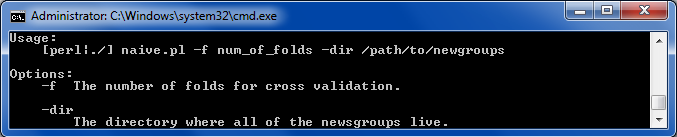
\includegraphics[scale=1]{usage.png}
\caption{Usage for naive.pl}
\end{figure}
\newpage
\section{Experiments}
\subsection{Computer Documents}
In the computer classes, I found a bunch of files that had BEGIN...END and "part x of y" blocks that appeared to have attachment files.  I realized these attachments were throwing my results way off for the computer class.  In Figure 3, I'm showing what these documents looked like if I kept the attachments in... basically resulting in gibberish.
\begin{figure}[h]
\begin{center}
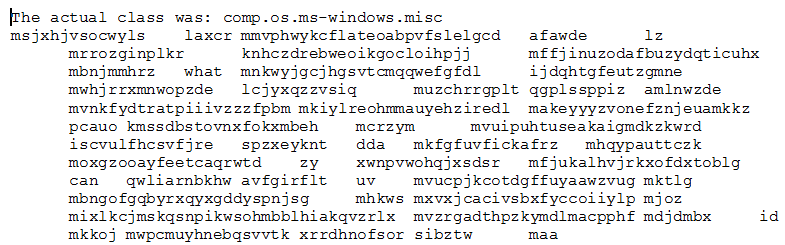
\includegraphics[scale=.8]{withattach.png}
\caption{Terms when the attachments are included in the computer class}
\end{center}
\end{figure}
\newline
After 22 pages of gibberish, we finally come to the scoring values--this is what Figure 4 shows.
\begin{figure}[h!]
\begin{center}
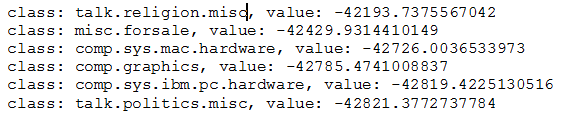
\includegraphics[scale=.8]{withattachscore.png}
\caption{Top 6 scores for including the attachments in the computer class}
\end{center}
\end{figure}
\newline
To remedy this problem, I implemented some regexes that captured when a BEGIN statement would start and end.  This resulted in much better results.
\begin{figure}[h]
\begin{center}
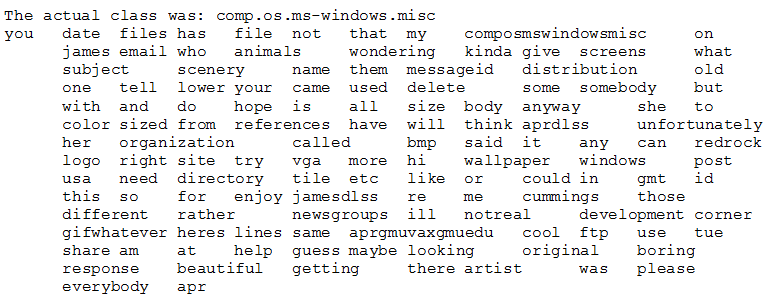
\includegraphics[scale=.8]{withoutattach.png}
\caption{Terms when the attachments aren't included in the computer class}
\end{center}
\end{figure}
\begin{figure}[h!]
\begin{center}
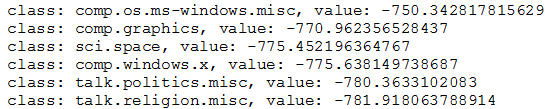
\includegraphics[scale=.8]{withoutattachscore.png}
\caption{Top 6 scores for not including the attachments in the computer class}
\end{center}
\end{figure}
\newline
As you can see from Figure 6, the results actually make more sense than before.  Instead of having extremely high values, we have relatively low ones that are getting similar classes for the given vocabulary.
\subsection{Politics}
The politics documents did extremely well, and it was interesting to see the classes that bubbled to the top with the given vocabulary.  Figure 7 gives an example of these results.
\newpage
\begin{figure}[ht]
\begin{center}
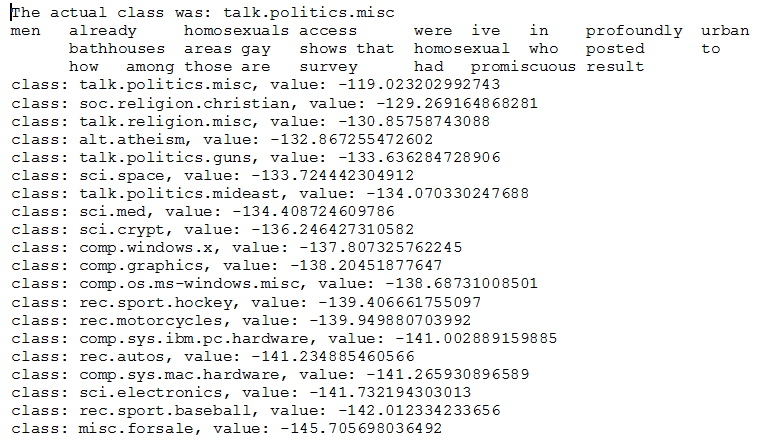
\includegraphics[scale=.8]{talkspolitics.png}
\caption{The classifications list for a talks.politics.misc document}
\end{center}
\end{figure}
\noindent
Not only did the algorithm predict the right class, but classes like forsale, sports, and computers are closer to the bottom, whereas classes like politics and religion are at the top.  These results make sense because given the vocabulary at the top of Figure 7, you would see terms like this come up in politics and religion, but most likely not in forsale or computers.
\section{Conclusion}
Overall, this algorithm did extremely well, and I was surprised to see the results that I got.  I can get around 70\% accuracy each time the algorithm runs.  However, this accuracy isn't an accurate result.  When the accuracy is lower, it's because the class that is chosen isn't necessarily "wrong."  The program is just picking what it thinks is the best based off of the probability of words that occur in each set.  To me, this seems like it might pick a better classification.
\newline\newline
The algorithm doesn't seem to single out one classification--they all seem to perform with the same accuracy.  It's all probabilistic, so given a proper test vocabulary--meaning it's not a short email that says something like, "Yes, I'll be there."--you're more than likely to get a reasonable result.
\newpage
\section{Code}
\lstset{language=perl,
stringstyle=\color{Orange},
keywordstyle=\color{Blue},
commentstyle=\color{Green},
showstringspaces=false
}
\lstinputlisting[language=perl]{naive.pl}
\end{document}